To explore the performance limits in actual operational conditions, the
\textit{slo-mo} results can be compared with the ones generated at
normal speed. Performance differences may point to potential source of
improvement by establishing modifications that nullify them.
We run these three algorithm at normal speed five times on each sequence.
We also applied two additional ORB-SLAM modifications that aim to lower
the compute time of the front-end computations 
\cite{zhao2018good2,zhao2019maphash} (time improvements can be seen in
Fig.~ \ref{fig:latency}).  The results are summarized on the right side of 
Table~\ref{tab:accuracy_summary}. 
To communicate tracking accuracy and the number of tracking failures, 
we compute the average tracking error only over successful cases, but 
mark the error in different gray levels according to failure quantity. 

Two of the three algorithms experience performance degradation to different
degrees when operating with time limit. One, SVO, did not significantly
change.  Though one additional sequence (\textit{outdoor4})was tracked
for one out of five runs, it did experience more failure than success.
Thus, we consider the change in track success rate to be negligible. The
tracking accuracy was within 2\% of the \textit{slo-mo} version. DSO
exhibits track loss for some sequences 
(\textit{room3}, \textit{outdoors4}, \textit{MH 05 diff}) relative to
\textit{slo-mo} which might also point to degradation of the back-end
processing due to the time constraints.  Further analysis would be
necessary to understand the source of these differences.
ORB degrades the most when returning back to normal speed, both in terms
of increased track failure and higher pose error. The higher time cost
of ORB-SLAM impacts performance, as ORB-SLAM has to skip frames to
complete the process initiated from an earlier one but not yet completed.
To examine the impact of lower latency two addtional low-latency algorithms, 
GoodFeature~\cite{zhao2019tro} and MapHash~\cite{zhao2019maphash} are
evaluated for comparison. 
Both were implemented in the ORB-SLAM framework and achieve low tracking
latency through different strategies. The former employs active matching
and the second employs more efficient local map subset selection. 
By lowering the pose tracking latency, the two algorithms improve
somewhat tracking success. A bigger improvement is seen for the pose
accuracy.

\begin{figure}[!t]
	\centering
	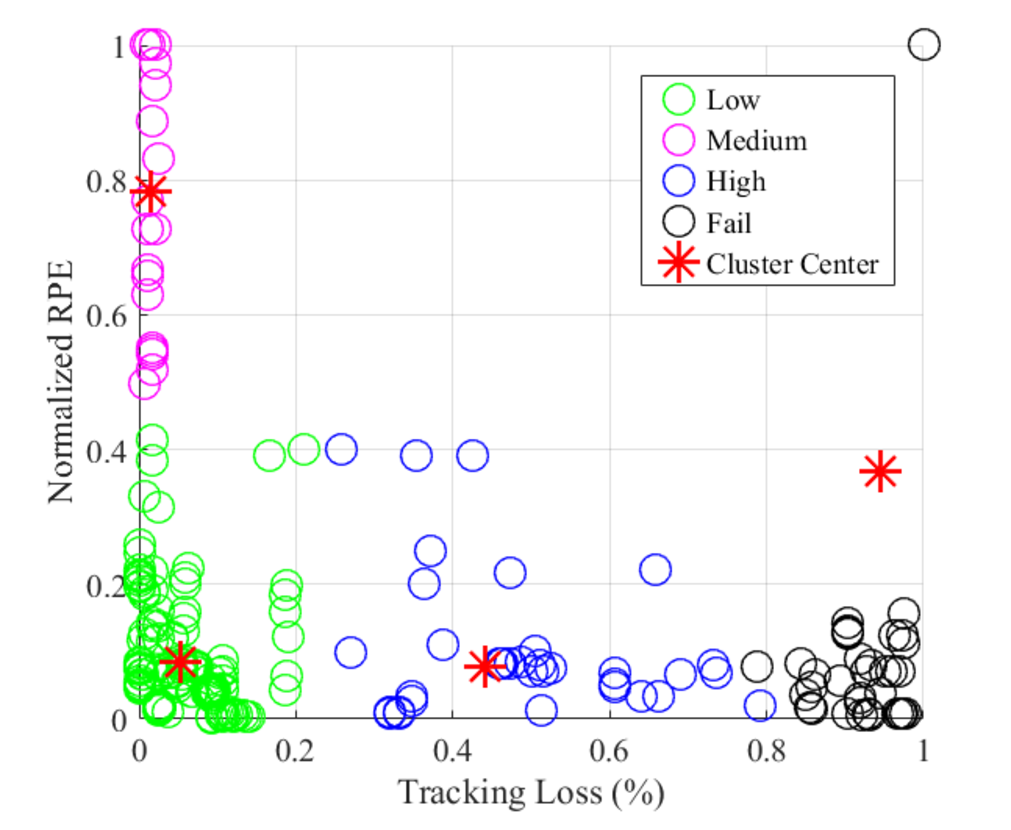
\includegraphics[width=0.9\linewidth]{./clustering2.pdf} \\
	\caption{Kmeans++ clustering on pose tracking errors.
 \label{fig:clustering}}
\end{figure}

\begin{figure*}[th!]
  \centering
\subfloat[DSO\label{fig:retrain_dso}]
        {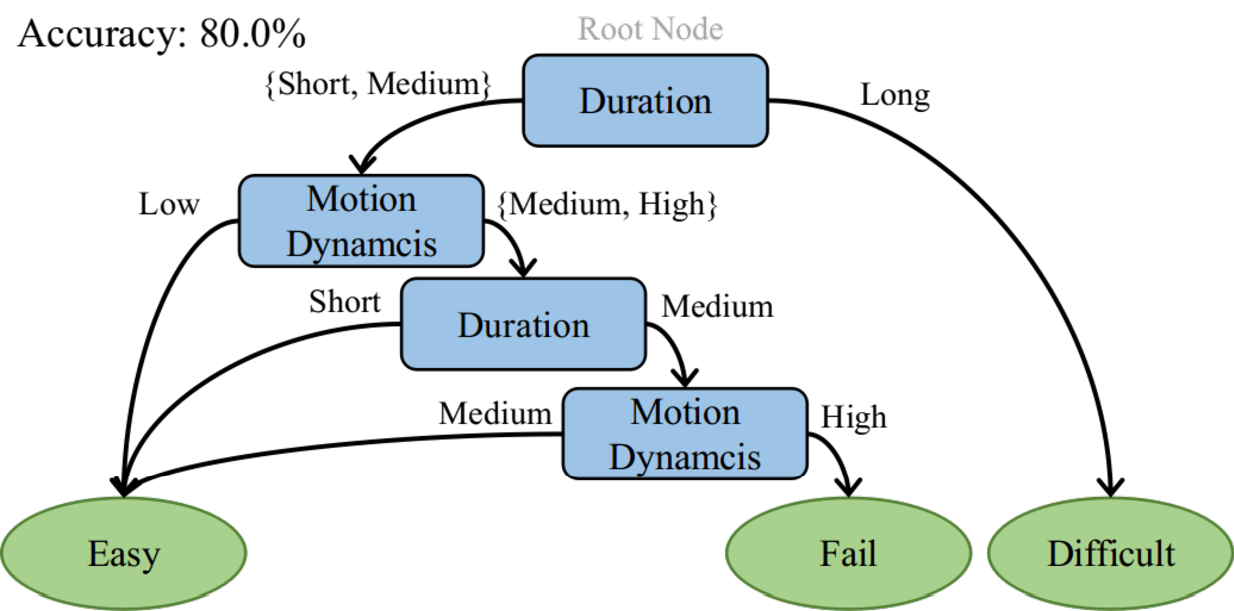
\includegraphics[width=0.8\columnwidth]{train_dso_quantatively2.pdf}}
    \qquad
\subfloat[SVO \label{fig:retrain_svo}]
        {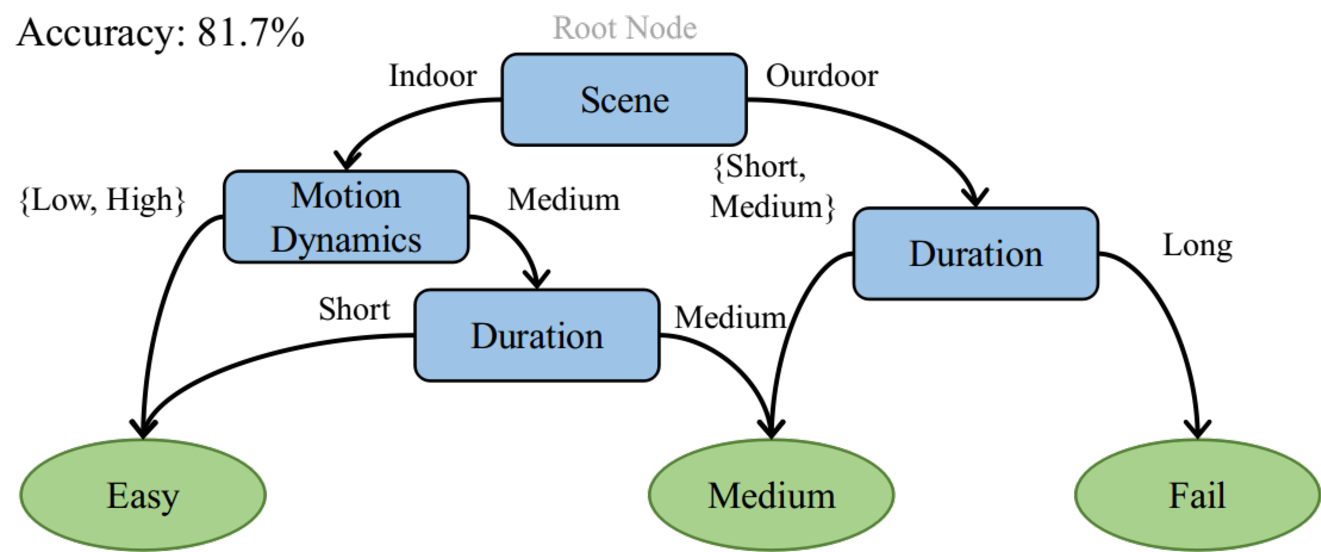
\includegraphics[width=0.8\columnwidth]{train_svo_quantatively2.pdf}}
\\
\subfloat[ORB \label{fig:retrain_orb}]
        {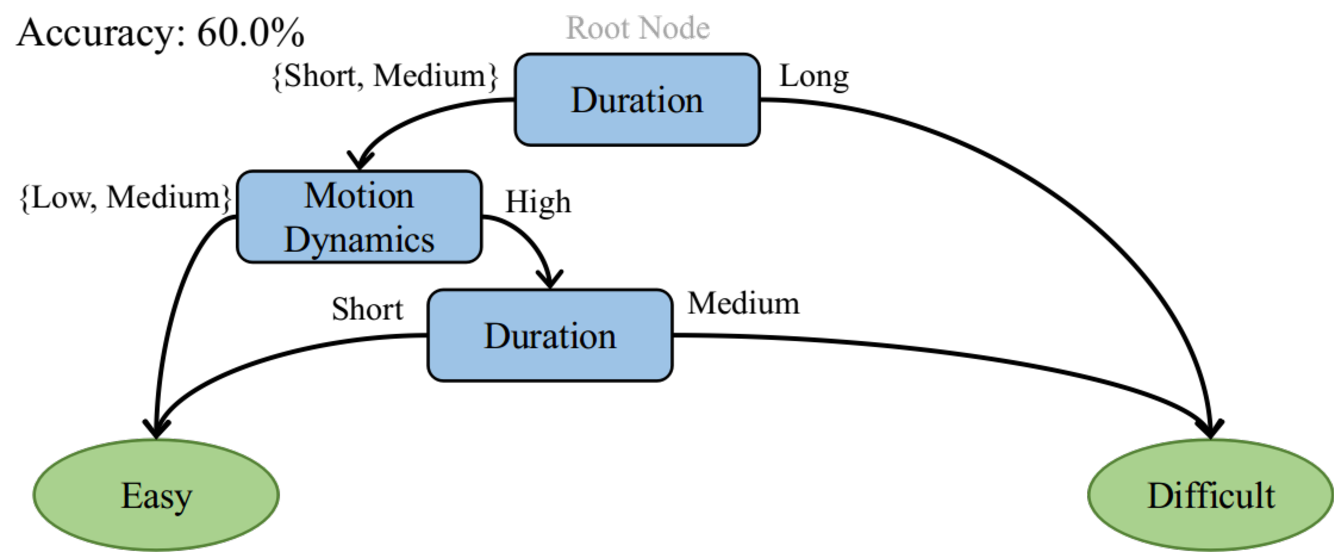
\includegraphics[width=0.8\columnwidth]{train_orb_quantatively2.pdf}}
            \qquad
\subfloat[ALL \label{fig:retrain_all}]
        {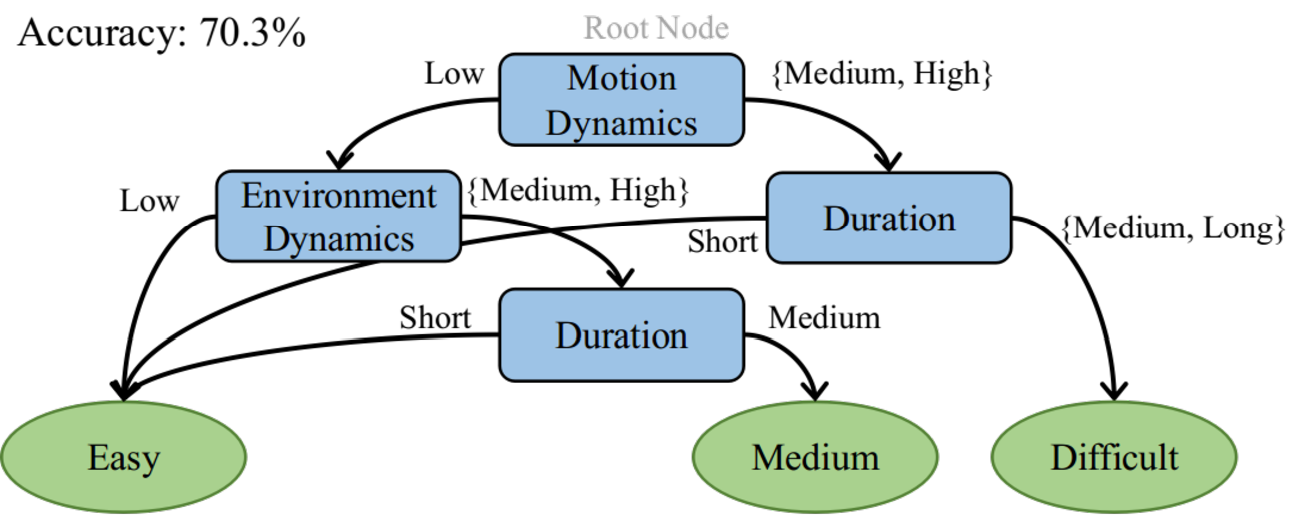
\includegraphics[width=0.8\columnwidth]{train_all_quantatively.pdf}}
\caption{Trained decision trees using pose tracking errors.} \label{fig:finaltrees}
\end{figure*}


While it is important to understand how well given visual SLAM algorithm
work in terms of relative standings, a better understanding or
characterization of performance would illuminate where additional effort
should be spent improving a particular SLAM algorithm. 
Here, we replicate the exploration of benchmark properties of 
Section~\ref{sec:bench} but use the quantitative outcomes from the
selected sequences.  In particular, we re-annotate the
\textit{Difficulty} label based on the track loss rate and the tracking
accuracy.
Each run with each algorithm on each sequence is taken as an observation, thus 
there will be 300 two-dimensional observations in total for training. 
To prevent biasing, we saturate RPE at 2 m/s and normalize the values. 
These two factors yield four candidate categories. 
An algorithm performance is considered as \textit{high} if it can track poses 
with low loss and low RPE. 
If it tracks the entire sequence but with poor accuracy, we consider
performance to be \textit{medium}. 
Moreover, we mark the performance as \textit{difficult} if it fails to track 
sometime in the middle of the sequence, and mark them as \textit{fail} if it 
is lost in the begining, no matter how accurately it tracks. 
K-means++\cite{arthur2007k} is applied to cluster observations into these four categories. The distribution of observations and the clustered centroids are 
shown in Fig~\ref{fig:clustering}. 

Given the cluster results, we categorize the pose tracking performance and 
build a decision tree for the three main SLAM algorithms tested. 
Since the tracking results are generated only from three VO algorithms,
the property \textit{Revisit Frequency} is removed as a factor.
The tree strucuture, from top to bottom, can indicate the significance
of sequence properties to each algorithm. 
According to Fig~\ref{fig:finaltrees}, these algorithms act differently
in terms of the selected characteristic sequences. 
For SVO, \textit{Scene} is the most important factor for decent operation, 
and \textit{Motion Dynamics} and \textit{Duration} come in the second place. 
No \textit{Difficult} leaf node exists, meaning that SVO usually tracked all 
the way if it is successfully started. 
The \textit{Medium} leaf node is connected with two \textit{Duration}
middle nodes, indicating its tracking accuracy depends to a great extent
on the sequence length. 
An interesting insight for DSO and ORB is their similarity. 
Their upper structures are basically the same, from \textit{Duration}, \textit{Motion Dynamics} to \textit{Duration}, which might partially explain the reason they can obtain competitive tracking accuracy on selected sequences.
The difference lies in the last judgement for \textit{Motion Dynamics}, where 
DSO can handle \textit{Medium} dynamics but will fail when it is \textit{High}. 
In contrast, ORB is not affected by \textit{Motion Dynamics} at this point, 
and no related failure will be caused. 
In summary, all algorithms as sensitive to \textit{Duration}, which is 
related to map maintenance, environment changes, and drift correction if
a loop closure module is available. 

In addition to the algorithm-specific decision trees, we aggregated all
of the data to generate a decision tree. 
Similar pre-process, clustering and training steps were conducted with the 
entire set, but with clustering into three categories. 
The generated decision tree is displayed on the lower right of
Fig~\ref{fig:finaltrees}. 
This tree is a quantitative vesion of the tree from Section~\ref{sec:bench}, 
based on actual outcomes as opposed to subjectively determined labels.
By comparison we can find that, both trees take the \textit{Motion Dynamics} as 
the first important factor, then comes \textit{Duration} and other factors. 
Our knowledge about what SLAM can do and what scenarios it can complete
is consistent with the quantative truth. 
A more comprehensive understanding can be obtained if breaking the
sequence properties into finer scale, but this comparion presents at
least two promising fields that SLAM research can focus on in the near
future: 
1) the robustness under aggressive motion patterns and 
2) the ability to handle long-term operation.
The former is usually handled by visual-inertial SLAM methods, to which
the same analysis can be applied.  The latter will require developing a
quantitative analysis methodology to better establish how to improve
long-term operation.







